\thispagestyle{empty}
\setlength{\unitlength}{1mm}
\makeatletter
\if@twoside%
    \noindent\begin{picture}(0,0)(1,-1)
    \put(-16.3,-265){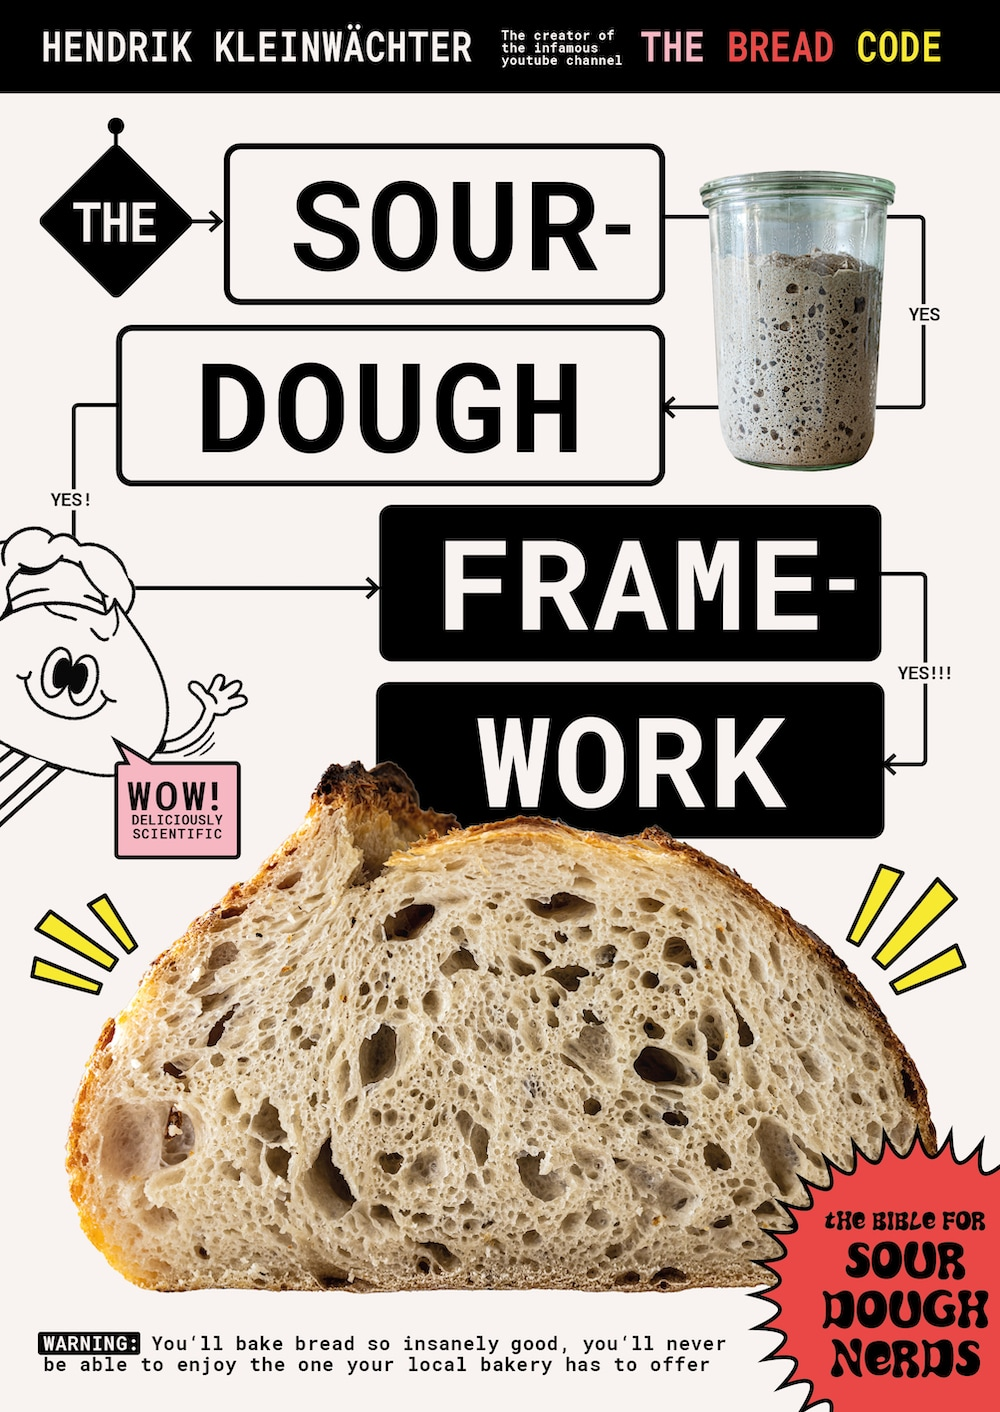
\includegraphics[width=1.33\linewidth]{cover/cover-page.jpg}}
    \end{picture}
\else%
    \noindent\begin{picture}(0,0)(1,-1)
    \put(-23.3,-265){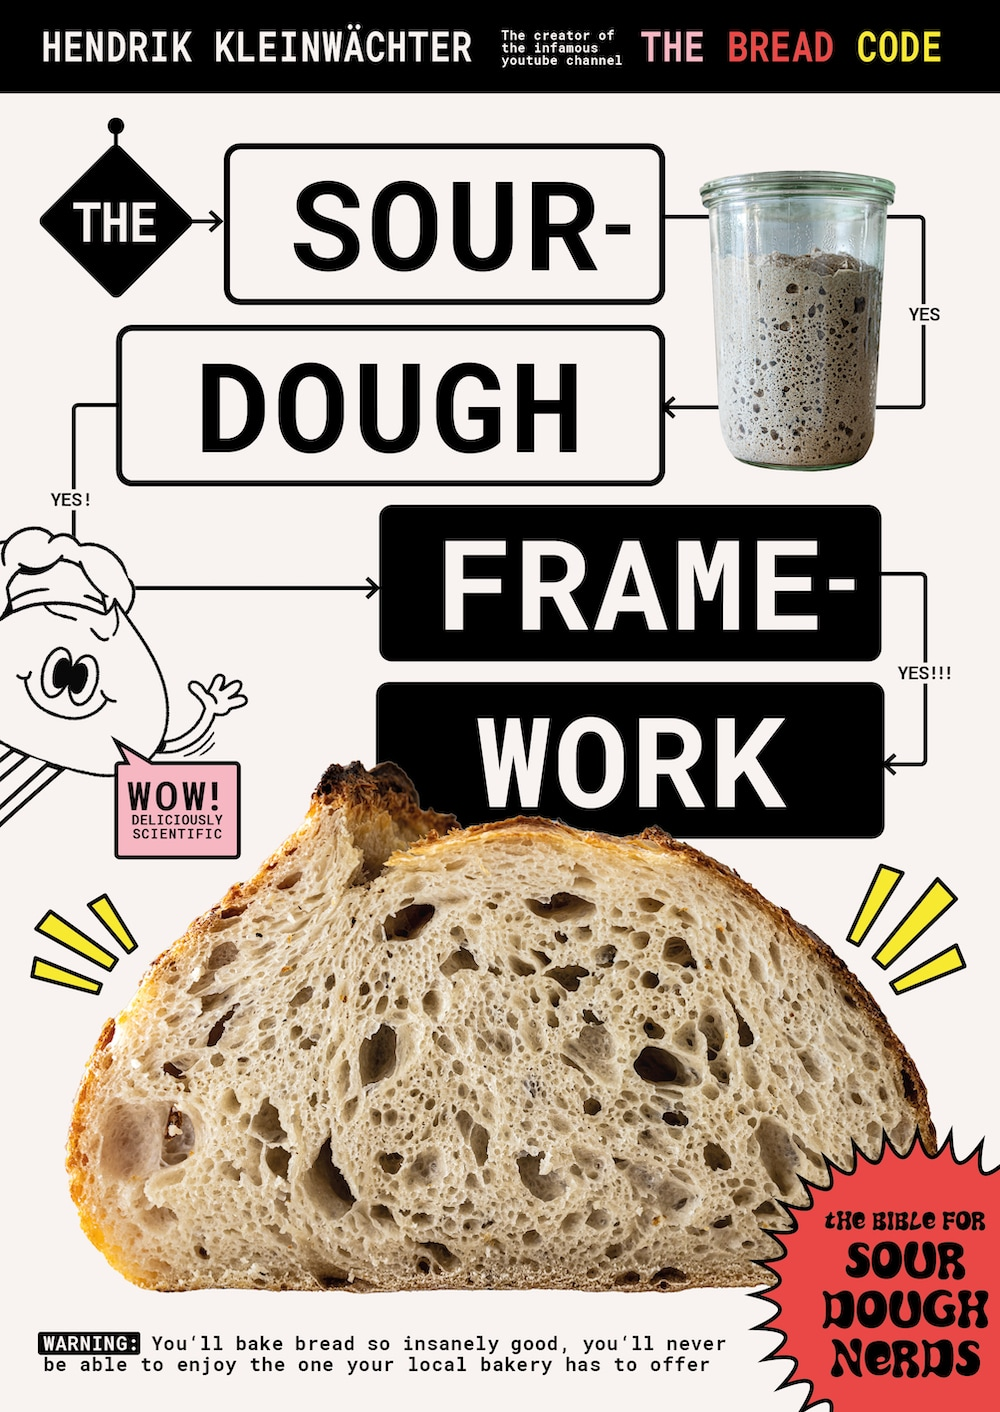
\includegraphics[width=1.33\linewidth]{cover/cover-page.jpg}}
    \end{picture}
\fi%
\makeatother

\newpage
\thispagestyle{empty}

\rule{1pt}{\textheight} % Vertical line
 % Whitespace between the vertical line and title page text
\hspace{0.05\textwidth}
 % Paragraph box for holding the title page text, adjust the width to move the
% title page left or right on the page
%\raggedleft%
\parbox[b]{0.75\textwidth}{%
{\Huge\bfseries The Sourdough Framework}\\[2\baselineskip] % Title
{\large\textit{Version: \today}}\\[4\baselineskip]
{\Large\textsc{Hendrik Kleinwächter}} % Author name, lower case for consistent small caps

% Whitespace between the title block and the copyright text
\vspace{0.5\textheight}


{\noindent
\begin{flushleft}
    
\includegraphics[width=3cm]{cover/CC-BY-SA}\par
The full source code for the book is available at
\url{https://github.com/hendricius/the-sourdough-framework/} under CC-BY-SA
license.
See \url{https://creativecommons.org/licenses/by-sa/4.0/} for more details.
Do not hesitate to report mistakes or sug\-gestions for
improvements. A hardcover version of the book is also available. More
information here: \url{https://www.breadco.de/hardcover-book}
\end{flushleft}
}
}
